\chapter{Non-Volatile Memory Integration in MPI-IO} \label{chap: deeper}

\section{Introduction}
\label{sec: motivation}
High Performance Computing (HPC) applications process large amounts of data that have to be written (read) to (from) large shared files residing in the global parallel file system. In order to make large datasets manageable, these are 
usually partitioned into smaller sub-sets and assigned to available cores for parallel processing. Complex datasets such as N-dimensional arrays are logically flattened into a linear sequence of bytes and striped across several I/O targets 
for best performance. This results in the loss of the original spatial locality, as shown in Figure~\ref{fig: small-io}.

\begin{figure}[!htb]
\centering
\includegraphics[width=\textwidth]{chapters/chapter3/figures/small-io}
\caption{Example of how a 3-Dimensional dataset is represented logically in the file as a sequence of bytes and how it is finally translated in the parallel file system.}
\label{fig: small-io}
\end{figure}

Due to this characteristic, accesses to spatially contiguous regions translate into non-contiguous accesses to the file. Therefore, applications generating a large number of small, non-contiguous I/O requests to the parallel file system 
usually experience degradation of I/O performance. Such performance degradation is known as the `small I/O problem' and is related to the fact that parallel file systems provide best I/O bandwidth performance for large contiguous requests, 
while they typically provide only a fraction of the maximum available bandwidth in the opposite case~\cite{ChingCLP06}~\cite{HeSSYT11}. This is due to the large number of Remote Procedure Calls (RPCs) generated by the file system clients 
overwhelming I/O servers, the resulting high number of hard disk head movements in every I/O target (seek overhead) and, ultimately, to the restrictions imposed by the POSIX I/O write semantic that generates lock contention in the file 
systems' blocks.

Having recognised the small I/O problem, collective I/O was proposed by the MPI-IO community~\cite{ThakurGL99}. Collective I/O exploits global I/O knowledge in parallel I/O to a shared file. This knowledge is used to build an aggregated view 
of the accessed region in the file and coalesce all the corresponding small non-contiguous requests into a smaller number of large contiguous accesses, later issued to the parallel file system. File system accesses are orchestrated in such a 
way that only a subset of the available processes actually performs I/O. These processes are called `aggregators', because they gather and aggregate all the requests on behalf of the other processes, whose only role in this case is to send 
(receive) data to (from) aggregators.

In conclusion, collective I/O can convert many small random accesses into large sequential accesses to the I/O subsystem, reducing the actual number of I/O requests that need to be accounted for by the I/O stack. Even when processes generate 
large I/O requests, it might be still beneficial to coordinate them to reduce parallel file system block locking contention as well as concurrency level on data servers. This mechanism effectively adapts the I/O pattern to the characteristics 
of the file system, extracting maximum performance from it.
Figure~\ref{figure: coll_io} exemplifies the basic collective I/O mechanism just described. In the figure there are six processes, four of which play the role of aggregators. Collective I/O proceeds in two phases: `data shuffling' and `data I/O'. 
Data shuffling takes place between all the processes and aggregators and is aimed to build the logically contiguous file regions (or file domains) that will be later accessed during the data I/O phase.

Two phase I/O has a number of problems that limit its scalability. The main issues are: (\textbf{a}) global synchronisation overhead between processes exchanging data, where I/O is bottlenecked by the slowest aggregator process~\cite{WeikuanV08}, 
(\textbf{b}) aggregators' contention on file system stripes (primarily due to stripe boundary misalignment of the file domains and the underlying file system locking mechanism\footnote{In current ROMIO versions the ADIO driver for Lustre can 
detect and align file domains to stripe boundaries thus avoiding stripe collisions. A new ADIO driver for BeeGFS supporting the same functionality has been developed in the course of this work.})~\cite{LiaoA08}, (\textbf{c}) aggregators' 
contention on I/O servers (related to inefficient file domain partitioning strategy), (\textbf{d}) pressure that large collective buffers can have on the memory system (due to scarce amount of available memory per single core in current and 
future large scale HPC clusters), and (\textbf{e}) high memory bandwidth requirements due to the large number of data exchanges between processes and aggregators~\cite{YinYTY12}. There is also a mismatch between logical file layouts and the 
collective I/O mechanism, which does not seem to take the physical data layouts into consideration~\cite{YongXTRG11}~\cite{XuechenJD09}.

\begin{figure}[!htb]
  \centering
  \includegraphics[width=0.6\textwidth]{chapters/chapter3/figures/coll-io}
  \caption{Collective I/O write example. A data set is partitioned and assigned to six processes. Four of them work as aggregators writing data to the global file system.}
  \label{figure: coll_io}
\end{figure}

Nowadays solid state drives (SSDs) are becoming more affordable and many HPC systems provide SSDs attached to compute nodes. Despite the fact that these devices formally provide an additional tier in the storage hierarchy, they are mostly used to 
store local data and rarely exploited for parallel I/O. As part of the Exascale10 (E10)~\cite{e10} initiative in the DEEP-ER~\cite{deep-er} project, we explore the benefits that the usage of such fast devices can bring when writing collectively to a 
shared file.

We integrate local storage resources attached to compute nodes (non-volatile memory devices) as persistent cache layer in ROMIO, providing all the additional infrastructure required to asynchronously flush the content of the cached data to the global file 
system, while keeping the MPI-IO consistency semantics. The new persistent cache layer is fully integrated inside ROMIO and can be easily accessed through a set of newly defined MPI-IO hints.

We show how when using local SSDs, if the number of aggregators is selected properly, significantly better I/O performance can be achieved compared to the case in which only the global file system is used. Contrarily, if the number of aggregators is not 
properly selected, I/O performance can even degrade. The additional cache layer also delivers more stable response times, reducing the impact of global synchronization on collective I/O, thus addressing point (\textbf{a}) previously discussed, and can reduce 
the memory pressure in systems with scarce amounts of main memory per core, thus addressing point (\textbf{d}).

The remainder of this chapter is organised as follows. In Section~\ref{sec: concept} we present the concept and design of the ROMIO caching layer and the new hints extensions supporting it, along with all the corresponding semantics implications, in 
Section~\ref{sec: evaluation} we show the benefits of collective I/O using different benchmarks, in Section~\ref{sec: related} we present collective I/O related works and finally in Section~\ref{sec: conclusion} we draw conclusions and discuss future 
developments.

\section{Concept \& Design}
\label{sec: concept}
In this section we present the high-level architecture of the current ROMIO implementation as well as our proposed architecture. The two are shown in Figure~\ref{figure: romio-architecture} and~\ref{figure: new-romio-architecture} respectively. The ROMIO 
middleware is designed to be modular and easily extensible. Support for different parallel file systems is provided through additional software modules called drivers. The appropriate driver is selected at file open time through an interface called Abstract 
Device I/O (ADIO), following an approach similar to the Virtual File System layer of the Linux Kernel. 

\begin{figure}[!htb]
  \centering
  \begin{subfigure}[t]{0.38\textwidth}
  \includegraphics[width=\textwidth]{chapters/chapter3/figures/romio-architecture-src.pdf}
  \caption{ROMIO architecture}
  \label{figure: romio-architecture}
  \end{subfigure}
  \begin{subfigure}[t]{0.55\textwidth}
  \includegraphics[width=\textwidth]{chapters/chapter3/figures/new-romio-architecture-src.pdf}
  \caption{Proposed ROMIO architecture}
  \label{figure: new-romio-architecture}
  \end{subfigure}
\end{figure}

In Figure~\ref{figure: romio-architecture} there are three different file system drivers: \textit{ad\_gpfs} for GPFS support, \textit{ad\_ufs} for Universal File System (UFS) support, and \textit{ad\_lustre} for Lustre support. These drivers share features 
implemented in the \textit{common} module. The common module contains the implementation for most of the I/O operations used by the UFS driver (ad\_ufs) and other drivers. File system drivers can implement their own I/O operations or use the ones made available 
by the common module. Lustre, for example, uses the common collective open operation (\codeword{ADIOI\_GEN\_Opencoll()}) but implements its own collective write operation (\codeword{ADIOI\_LUSTRE\_WriteStridedColl()}) described in Figure~\ref{figure: coll_io_impl}. 
Specific implementations are selected using a file operation table that has to be defined by every file system driver. Listing~\ref{list: lustre_table} shows the operation table for the ad\_lustre driver.

\begin{lstlisting}[language=C, caption=Operation Table for Lustre Driver, label={list: lustre_table}]
struct ADIOI_Fns_struct ADIO_LUSTRE_operations = {
    ADIOI_LUSTRE_Open, /* Open */
    ADIOI_GEN_OpenColl, /* OpenColl */
    ADIOI_LUSTRE_ReadContig, /* ReadContig */
    ADIOI_LUSTRE_WriteContig, /* WriteContig */
    ADIOI_GEN_ReadStridedColl, /* ReadStridedColl */
    ADIOI_LUSTRE_WriteStridedColl, /* WriteStridedColl */
    ADIOI_GEN_SeekIndividual, /* SeekIndividual */
    ADIOI_GEN_Fcntl, /* Fcntl */
    ADIOI_LUSTRE_SetInfo, /* SetInfo */
    ADIOI_GEN_ReadStrided, /* ReadStrided */
    ADIOI_LUSTRE_WriteStrided, /* WriteStrided */
    ADIOI_GEN_Close, /* Close */
#if defined(ROMIO_HAVE_WORKING_AIO) && !defined(CRAY_XT_LUSTRE)
    ADIOI_GEN_IreadContig, /* IreadContig */
    ADIOI_GEN_IwriteContig, /* IwriteContig */
#else
    ADIOI_FAKE_IreadContig, /* IreadContig */
    ADIOI_FAKE_IwriteContig, /* IwriteContig */
#endif
    ADIOI_GEN_IODone, /* ReadDone */
    ADIOI_GEN_IODone, /* WriteDone */
    ADIOI_GEN_IOComplete, /* ReadComplete */
    ADIOI_GEN_IOComplete, /* WriteComplete */
    ADIOI_GEN_IreadStrided, /* IreadStrided */
    ADIOI_GEN_IwriteStrided, /* IwriteStrided */
    ADIOI_GEN_Flush, /* Flush */
    ADIOI_GEN_Resize, /* Resize */
    ADIOI_GEN_Delete, /* Delete */
    ADIOI_GEN_Feature, /* Features */
    "LUSTRE:",
};
\end{lstlisting}

In Figure~\ref{figure: new-romio-architecture} we extend the presented ROMIO architecture with two additional modules: a dedicated driver supporting the BeeGFS file system (\textit{ad\_beegfs}) and a \textit{cache plugin} that links directly to the
common module, thus providing NVM caching features to all the underlying file system drivers. We also developed an external library called \textit{MPIWRAP} that is used to allow transparent integration of the new caching functionalities into existing 
applications without any need of modifying them. 

In the rest of the chapter we describe in details the new MPI-IO hints supporting local NVM caching and the corresponding cache plugin module implementation.

\subsection{MPI-IO Hints Extensions}
To take advantage of attached non-volatile memories in computing nodes we introduced a new set of MPI-IO hints, reported in Table~\ref{table: hints_table}, and a corresponding set of modifications in the ROMIO implementation of the UFS driver 
supporting them.

\begin{table}[!htb]
\centering
\ra{1.5}
\caption{Proposed MPI-IO hints extensions.}
\newcolumntype{K}{>{\centering\arraybackslash} m{4cm}}
\newcolumntype{V}{>{\centering\arraybackslash} m{5cm}}
\begin{tabular}{KV}
\toprule
\bf \small Hint & \bf \small Value \\
\midrule
\small \codeword{e10\_cache} & \small \codeword{enable}, \codeword{disable}, \codeword{coherent}\\
\small \codeword{e10\_cache\_path} & \small cache directory pathname\\
\small \codeword{e10\_cache\_flush\_flag} & \small \codeword{flush\_immediate}, \codeword{flush\_onclose}, \codeword{flush\_none}\\
\small \codeword{e10\_cache\_discard\_flag} & \small \codeword{enable}, \codeword{disable}\\
\small \codeword{e10\_cache\_threads} & \small number of synchronisation thread in pool\\
\small \codeword{ind\_wr\_buffer\_size} & \small synchronisation buffer size [bytes]\\
\hline
\end{tabular}
\label{table: hints_table}
\end{table}

The new hints are used to control the data path in the storage system as well as to define a basic set of cache policies for synchronisation and space management. In particular, the \codeword{e10\_cache} hint is used to \codeword{enable} or 
\codeword{disable} the cache, directing applications' data to the local file system instead of the global file system. When the hint is set to \codeword{coherent} all the written data extents will be locked until cache synchronisation is completed. 
The \codeword{e10\_cache\_path} hint is used to control where, in the local file system tree, the cache file will reside. The \codeword{e10\_cache\_flush\_flag} hint is used to control the synchronisation policy of cached data to the global file. 
If the hint is set to \codeword{flush\_immediate} data will be immediately flushed to the global file. Alternatively, if the hint is set to \codeword{flush\_onclose} data will be flushed to the global file when it is closed. A \codeword{flush\_none} 
option is also provided to keep data local to the node and never flush it to the global file system. The \codeword{e10\_cache\_discard\_flag} hint is used to perform basic cache space management. In particular, if the hint is set to \codeword{enable} 
the cache file will be removed after the file is closed, otherwise (\codeword{disable}) it will be retained until the user manually removes it. The \codeword{e10\_cache\_threads} hint is used to communicate the implementation the number of threads 
that need to be created in the synchronisation thread pool when the file is opened (default is 1). Finally, the \codeword{ind\_wr\_buffer\_size} hint controls the size of the buffer used to synchronise cached data to the global file. This hint already 
existed in ROMIO but was only used during independent I/O to determine the write granularity. The hints in Table~\ref{table: hints_table} can be used in conjunction with the collective I/O hints described in section~\ref{subsec: hints}.

Besides the proposed cache policies, more complex ones are possible. For example, the cache synchronisation could take into account the level of congestion of the I/O servers. The cache replacement policy could also use a more complex strategy to 
evict cached files (or extents of data inside the file). Although these can be implemented in ROMIO, they introduce more sophisticated functionalities that go beyond the scope of this work.

\subsection{Cache Hints Integration in ROMIO}
\label{subsec: support}
As already mentioned, the introduced MPI-IO hints are supported by a corresponding set of modifications in the ROMIO implementation~\cite{E10-DEEPER} in the form of cache plugin. These modifications, following described, provide the functionalities 
necessary to handle the additional cache layer.

\subsubsection{Cache Synchronisation Request}
\label{subsubsec: cache-sync-req}
The \codeword{ADIOI\_Sync\_req\_t} object provides the infrastructure required to initialise/finalise, set/get attributes to/from synchronisation requests. Synchronisation requests are initialised by the main thread in the write function and submitted 
to a separate thread (synchronisation thread) which will satisfy them while the main thread can progress with useful work. Listing~\ref{list: sync-req} shows the object API.

\begin{lstlisting}[language=C, caption=Synchronisation Request API, label={list: sync-req}]
/* for ADIOI_Sync_req_{get,set}_key() */
enum {
  ADIOI_SYNC_TYPE = 0, /* sync req type        */
  ADIOI_SYNC_OFFSET,   /* sync req write off   */
  ADIOI_SYNC_DATATYPE, /* sync req datatype    */
  ADIOI_SYNC_COUNT,    /* sync req count       */
  ADIOI_SYNC_REQ,      /* sync req MPI_Request */
  ADIOI_SYNC_ERR_CODE, /* sync req error_code  */
  ADIOI_SYNC_FFLAGS,   /* sync req flush flag  */
  ADIOI_SYNC_ALL,      /* sync req all fields  */
  ADIOI_SYNC_REQ_ERR   /* sync req err code    */
};

struct ADIOI_Sync_req {
  int           type_;
  int           count_;
  int           error_code_;
  int           fflags_;
  ADIO_Offset   off_;
  MPI_Datatype  datatype_;
  ADIO_Request *req_;
};

/* Synchronisation Request Interfaces */
typedef struct ADIOI_Sync_req *ADIOI_Sync_req_t;

int ADIOI_Sync_req_init(ADIOI_Sync_req_t *, ...);
int ADIOI_Sync_req_init_from(ADIOI_Sync_req_t *, 
  ADIOI_Sync_req_t);
int ADIOI_Sync_req_fini(ADIOI_Sync_req_t *);
int ADIOI_Sync_req_get_key(ADIOI_Sync_req_t, ...);
int ADIOI_Sync_req_set_key(ADIOI_Sync_req_t, ...);
\end{lstlisting}

There are two types of synchronisation requests, \codeword{ADIOI\_THREAD\_SYNC} and \codeword{ADIOI\_THREAD\_SHUTDOWN}. The first is used to describe a written file extent that needs to be copied from the cache to the global file system, 
the second is used to shut down the synchronisation thread when the file is closed.

Every synchronisation request has a \codeword{MPI\_Request} handle used to start asynchronous copy of data from the cache to the global file system and to check upon request completion by the main thread using \codeword{MPI\_Wait()}.

\subsubsection{Cache Synchronisation Thread}
\label{subsubsec: cache-sync-thread}
The \codeword{ADIOI\_Sync\_thread\_t} object provides the infrastructure to initialise/finalise threads and to enqueue, flush and wait for synchronisation requests. A pool of synchronisation threads is created when the file is opened and destroyed 
when the file is closed. Listing~\ref{list: sync-thread} shows the object API.

\begin{lstlisting}[language=C, caption=Synchronisation Thread API, label={list: sync-thread}]
enum {
  ADIOI_THREAD_SYNC = 0,
  ADIOI_THREAD_SHUTDOWN
};

struct ADIOI_Sync_thread {
  ADIO_File            fd_;
  pthread_t            tid_;
  pthread_attr_t       attr_;
  ADIOI_Atomic_queue_t sub_;
  ADIOI_Atomic_queue_t pen_;
  ADIOI_Atomic_queue_t wait_;
};

typedef struct ADIOI_Sync_thread *ADIOI_Sync_thread_t;

int  ADIOI_Sync_thread_init(ADIOI_Sync_thread_t *, ...);
int  ADIOI_Sync_thread_fini(ADIOI_Sync_thread_t *);
void ADIOI_Sync_thread_enqueue(ADIOI_Sync_thread_t, 
  ADIOI_Sync_req_t);
void ADIOI_Sync_thread_flush(ADIOI_Sync_thread_t);
void ADIOI_Sync_thread_wait(ADIOI_Sync_thread_t);
\end{lstlisting}

The synchronisation thread object has three queues, a pending queue (\textit{pen\_}), a submission queue (\textit{sub\_}) and a wait queue (\textit{wait\_}). New synchronisation requests are first added to the pending queue using the 
\codeword{ADIOI\_Sync\_thread\_enqueue()} function. Pending requests are not satisfied until they are moved to the submission queue using the \codeword{ADIOI\_Sync\_thread\_flush()} function. This function also pushes a copy of the request pointer 
to the wait queue, which is later used by the \codeword{ADIOI\_Sync\_thread\_wait()} function to wait for submitted requests to complete.

\subsubsection{Synchronisation Thread Pool Initialisation}
\label{subsubsec: thread-pool-init}
The thread pool is initialised in \codeword{ADIOI\_GEN\_Opencoll()}. This function is invoked by \codeword{MPI\_File\_open()} every time a new file is opened. Listing~\ref{list: open-coll} shows the code responsible for opening the cache file in the 
local file system and to start the synchronisation threads.

\begin{lstlisting}[language=C, caption=Synchronisation Thread Initialisation, label={list: open-coll}]
void ADIOI_GEN_Opencoll(...) {
  ...
  /* check cache mode */
  if (fd->hints->e10_cache == ADIOI_HINT_ENABLE) {
    /* get MPI_File handle for cache and init it */
    MPI_File mpi_fh = MPIO_File_create(sizeof(
      struct ADIOI_FileD));
    fd->cache_fd = MPIO_File_resolve(mpi_fh);
    fd->cache_fd->filename = ADIOI_GetCacheFilePath(
      fd->filename, fd->hints->e10_cache_path);
    fd->cache_fd->file_system = fd->file_system;
    fd->cache_fd->fns = fd->fns;
    fd->cache_fd->cache_fd = ADIO_FILE_NULL;

    ...

    /* every process tries opening the cache file */
    (*(fd->fns->ADIOI_xxx_Open))(fd->cache_fd,
      error_code);

    ...

    /* init synchronisation thread pool */
    if (*error_code == MPI_SUCCESS && 
        fd->hints->e10_cache_flush_flag != 
          ADIOI_HINT_FLUSHNONE) {
      if (fd->hints->cb_write == ADIOI_HINT_ENABLE)
        if (fd->is_agg)
          *error_code = 
            ADIOI_Sync_thread_pool_init(fd, NULL);
        else
          *error_code = MPI_SUCCESS;
      else
        *error_code = ADIOI_Sync_thread_pool_init(
          fd, NULL);
    }

    /* check every process has returned success */
    MPI_Allreduce(error_code, &max_error_code, 1, 
      MPI_INT, MPI_MAX, fd->comm);

    if (max_error_code != MPI_SUCCESS) {
      if (*error_code == MPI_SUCCESS ||
          *error_code == ADIOI_ERR_THREAD_CREATE) {
        (*(fd->fns->ADIOI_xxx_Close))(fd->cache_fd,
          error_code);
        if ((fd->cache_fd->access_mode & ADIO_CREATE) &&
            (fd->cache_fd->access_mode & 
              ADIO_DELETE_ON_CLOSE)) {
          ADIO_Delete(fd->cache_fd->filename, error_code);
        }
        /* fini synchronisation thread pool */
        if (fd->hints->e10_cache_flush_flag != 
            ADIOI_HINT_FLUSHNONE && fd->thread_pool) {
          ADIOI_Sync_thread_pool_fini(fd);
        }
      }

      /* Revert to standard file access: no cache */
      ADIOI_Info_set(fd->info, "e10_cache", "disable");
      fd->hints->e10_cache = ADIOI_HINT_DISABLE;
    } else {
      fd->cache_fd->is_open = 1;
    }
  }
  ...
}
\end{lstlisting}

In order for the implementation to exploit local NVM caching both local file creation and thread initialisation must succeed. The MPI file handle for the cache file is stored in \textit{cache\_fd} inside the file handle of the global file. 
When collective I/O is enabled only the aggregators will initialise the synchronisation thread pool. In any other case every process will do independent I/O and will thus initialise its own pool.

\subsubsection{Synchronisation Request Submission}
\label{subsubsec: sync-req-sub}
\codeword{ADIOI\_GEN\_WriteContig()} is the function responsible for writing data to the file. This function is used by both collective and independent I/O. We have extended the write function to support creation and submission of new synchronisation 
requests to the thread pool. Listing~\ref{list: req-sub} shows the corresponding implementation.

\begin{lstlisting}[language=C, caption=Synchronisation Request Submission, label={list: req-sub}]
void ADIOI_GEN_WriteContig(...) {
  ...

  /* if using the cache select the cache file handle */
  if (fd->cache_fd && fd->cache_fd->is_open) {
    fh = fd->cache_fd;

    /* if cache is coherent lock global file extent */ 
    if (fd->hints->e10_cache_coherent == ADIOI_HINT_ENABLE)
      ADIOI_WRITE_LOCK(fd, offset, SEEK_SET, len);
  }

  /* write to the cache file handle */

  /* init and submit sync request */
  if (fd->cache_fd && fd->cache_fd->is_open && 
      fd->hints->e10_cache_flush_flag != 
        ADIOI_HINT_FLUSHNONE) {
    ADIOI_Sync_req_t sub;
    int threads, curr_thread, idx;
    ADIO_Request *r = (ADIO_Request *)ADIOI_Malloc(
      sizeof(ADIO_Request));

    *r = MPI_REQUEST_NULL;
    threads = fd->hints->e10_cache_threads;
    curr_thread = fd->thread_curr;
    idx = curr_thread % threads;

    /* init sync req */
    ADIOI_Sync_req_init(&sub, ADIOI_THREAD_SYNC, offset, 
      datatype, count, r, 0);

    /* enqueue sync request to thread and flush */
    ADIOI_Sync_thread_enqueue(fd->thread_pool[idx], sub);
    if (fd->hints->e10_cache_flush_flag == 
        ADIOI_HINT_FLUSHIMMEDIATE)
      ADIOI_Sync_thread_flush(fd->thread_pool[idx]);

    /* select next thread in the pool */
    fd->thread_curr = (curr_thread + 1) % threads;
  }
}
\end{lstlisting}

For each write a new synchronisation request is initialised using the same set of I/O parameters (i.e. offset, datatype, count, etc) as the original write operation. The request is then enqueued to the appropriate thread in the pool using 
\codeword{ADIOI\_Sync\_thread\_enqueue()}. If the \codeword{e10\_cache\_flush\_flag} is set to \codeword{flush\_immediate} the request is immediately scheduled to be served by invoking \codeword{ADIOI\_Sync\_thread\_flush()}, otherwise it will be 
flushed when the file is closed.

\subsubsection{Cache Flushing}
\label{subsubsec: cache-flush}
\codeword{ADIOI\_GEN\_Flush()} is the function responsible for flushing the page cache. This function is used by \codeword{MPI\_File\_sync()}. We have extended the file flush function to support flushing and waiting of outstanding synchronisation 
requests. Listing~\ref{list: req-flush} shows the corresponding implementation.

\begin{lstlisting}[language=C, caption=Cache Flushing, label={list: req-flush}]
void ADIOI_GEN_Flush(...) {

  ...

  if (fd->cache_fd == NULL || fd->thread_pool == NULL ||
      (fd->cache_fd && !fd->cache_fd->is_open) ||
      (fd->cache_fd && fd->cache_fd->is_open &&
      fd->hints->e10_cache_flush_flag == ADIOI_HINT_FLUSHNONE))
    goto fn_flush;

  threads = fd->hints->e10_cache_threads;

  /* Flush all the requests in each thread */
  for (idx = 0; idx < threads; idx++) {
    ADIOI_Sync_thread_flush(fd->thread_pool[idx]);
  }

  /* Wait for submitted requests to complete */
  for (idx = 0; idx < threads; idx++) {
    ADIOI_Sync_thread_wait(fd->thread_pool[idx]);
  }
  return;

fn_flush:
  /* fsync global file handle */
}
\end{lstlisting}

When invoked, the flush routine will trigger cache synchronisation for every thread in the pool by invoking \codeword{ADIOI\_Sync\_thread\_flush()}. As previously described this will move all the requests in the pending queue to the submission queue to 
be served. If the pending queue is empty, the thread flush routine will return immediately. Once all the threads in the pool have been flushed, the routine waits on each of them to complete by invoking \codeword{ADIOI\_Sync\_thread\_wait()} and finally 
returns.

\subsubsection{Synchronisation Thread Pool Finalisation}
\label{subsubsec: thread-pool-fini}
\codeword{ADIO\_Close()} is the function responsible for closing a file. This function is used by \codeword{MPI\_File\_close()}. We have extended the close function to support closing of cache file and finalisation of the synchronisation thread pool. 
Listing~\ref{list: thread-fini} shows the corresponding implementation.

\begin{lstlisting}[language=C, caption=Synchronisation Thread Pool Finalisation, label={list: thread-fini}]
void ADIO_Close(...) {

  ...

  if (fd->cache_fd) {
    if (fd->cache_fd->is_open) {
      /* First check if there is any outstanding sync */
      (*(fd->fns->ADIOI_xxx_Flush))(fd, error_code);

      /* Afterwards we can close the cache file */
      (*(fd->fns->ADIOI_xxx_Close))(fd->cache_fd, 
        error_code);

      /* Finilise thread pool */
      ADIOI_Sync_thread_pool_fini(fd);
    }

    /* Only the process that created the file deletes it */
    if ((fd->cache_fd->access_mode & ADIO_CREATE) &&
        (fd->cache_fd->access_mode & ADIO_DELETE_ON_CLOSE))
      ADIO_Delete(fd->cache_fd->filename, &err);

    /* Free cache_fd */
    ADIOI_Free(fd->cache_fd->filename);
    MPIO_File_free(&(fd->cache_fd));
    fd->cache_fd = ADIO_FILE_NULL;
  }

  ...

}
\end{lstlisting}

When invoked, the close routine will trigger the flushing of the cache (\codeword{(*(fd->fns->ADIOI\_xxx\_Flush))()}), close the cache file (\codeword{(*(fd->fns->ADIOI\_xxx\_Close))()}) and finalise the thread pool (\codeword{ADIOI\_Sync\_thread\_pool\_fini()}).

\begin{figure}[!htb]
  \centering
  \includegraphics[width=\textwidth]{chapters/chapter3/figures/ext2ph+e10}
  \caption{New Collective I/O flow diagram.}
  \label{figure: new_coll_io_impl}
\end{figure}

Figure~\ref{figure: new_coll_io_impl} graphically shows the modified flow diagram for the new collective I/O implementation just described. Compared to Figure~\ref{figure: coll_io_impl}, there is now an additional component representing the synchronisation thread. 
When data is written to the cache file, a synchronisation request for the written data is initialised and submitted to the \codeword{ADIOI\_Sync\_thread\_t} object. The object's pthread continuously search in the submission queue (\textit{sub\_}) for new 
synchronisation requests to satisfy.

\subsection{BeeGFS Cache Integration in ROMIO}
The BeeGFS file system provides its own caching infrastructure, which includes a set of APIs to control the caching functionalities and a deamon process, running on the host machine, that takes care of moving data between the cache and the global 
file system. For this reason, some of the cache plugin features presented before for the universal file system module are redundant. In particular, we do not any longer need to manually open a cache file in the host and start a pool of synchronisation 
threads. When using the BeeGFS cache API the file system will take care of all these aspects for us. Nevertheless, we can still recycle some part of the cache plugin as described below.

\subsubsection{Cache Opening}
The BeeGFS collective open function is implemented in \codeword{ADIOI\_BEEGFS\_OpenColl()}. This will be automatically invoked when \codeword{MPI\_File\_open()} is called by the application. The implementation for the collective open is similar to the 
universal file system implementation and is reported in Listing~\ref{list: beegfs_opencoll}.

\begin{lstlisting}[language=C, caption=BeeGFS Collective Open Implementation, label={list: beegfs_opencoll}]
void ADIOI_BEEGFS_OpenColl(...) {

  ...

  /* workout parent directory for file */
  dir = ADIOI_Dirname(fd->filename);

fn_open:
  if (access_mode & ADIO_CREATE) {
    if (rank == fd->hints->ranklist[0]) {
      /* remove delete on close flag if set */
      if (access & ADIO_DELETE_ON_CLOSE)
        fd->access_mode = access_mode ^ 
                          ADIO_DELETE_ON_CLOSE;
      else
        fd->access_mode = access_mode;
      
      /* prefetch the parent dir into the cache */
      if (fd->hints->e10_cache == ADIOI_HINT_ENABLE) {
        ret = deeper_cache_prefetch(dir, 
                DEEPER_PREFETCH_SUBDIR | 
                DEEPER_PREFETCH_WAIT);

        /* enforce synchronous flush 
         * when closing the file */
        fd->cache_oflags = DEEPER_OPEN_FLUSHONCLOSE | 
                           DEEPER_OPEN_FLUSHWAIT;
      } else {
        ret = DEEPER_RETVAL_SUCCESS;
      }

      ...

      /* only the rank 0 process creates the file 
       * invoking deeper_cache_open() */
      if (ret == DEEPER_RETVAL_SUCCESS || 
           (ret == DEEPER_RETVAL_ERROR && errno == EEXIST)) 
      {
        (*(fd->fns->ADIOI_xxx_Open))(fd, error_code);
      }

      /* close the cache file forcing BeeGFS to flush it */
      if (*error_code == MPI_SUCCESS)
        (*(fd->fns->ADIOI_xxx_Close))(fd, error_code);

      MPI_Bcast(error_code, 1, MPI_INT, 
                fd->hints->ranklist[0], fd->comm);

      /* restore the delete on close flag if it was set */
      fd->access_mode = access_mode;
    } else {
      MPI_Bcast(error_code, 1, MPI_INT, 
                fd->hints->ranklist[0], fd->comm);
    }

    /* check cache errors and if any revert 
     * to standard I/O */
  }

  /* now every process opens the file */

  if (fd->hints->e10_cache == ADIOI_HINT_ENABLE) {
    deeper_cache_prefetch(dir, DEEPER_PREFETCH_SUBDIR |
                               DEEPER_PREFETCH_WAIT);

    /* default open flags */
    fd->cache_oflags = DEEPER_OPEN_FLUSHONCLOSE | 
                       DEEPER_OPEN_FLUSHWAIT;

    if (fd->hints->e10_cache_discard_flag == 
        ADIOI_HINT_ENABLE)
      fd->cache_oflags |= DEEPER_OPEN_DISCARD;

  }

  (*(fd->fns->ADIOI_xxx_Open))(fd, error_code);

  ...

}
\end{lstlisting}

Similarly to before, the rank 0 process needs to setup the cache by prefetching the file parent directory into the cache, through \codeword{deeper\_cache\_prefetch()}. Afterwards, rank 0 opens the file inside the prefetched directory 
by invoking the local open (\codeword{ADIOI\_BEEGFS\_Open()}). The local open performs the real open operation using \codeword{deeper\_cache\_open()} instead of \codeword{open()}. If the open succeeds the cache file is closed, thus 
forcing BeeGFS to mirror it in the global file system. At this point all the other processes can prefetch the parent directory and the file created by rank 0 inside it.

By default the cache open flags for the file, \codeword{fd->cache\_oflags}, are always set to DEEPER\_FLUSHONCLOSE and DEEPER\_FLUSHWAIT; this means that if there is any non-synchronised data in the cache, the close operation will force 
this data to be flushed to the global file system and will not return until all the data has been copied.

\subsection{Cache Consistency Semantics}
\label{subsec: consistency}
As far as write consistency is concerned, the MPI-IO interface does not make any assumption regarding the underlying storage system or its semantics. ROMIO specifically supports file systems that are both POSIX compliant, like Lustre, 
and non-POSIX compliant, like NFS or PVFS. In MPI-IO, written data becomes globally visible only after either \codeword{MPI\_File\_sync()} or \codeword{MPI\_File\_close()} are invoked on the MPI file handle and by default there is no write 
atomicity. The motivation is that data can be cached at some level locally in the compute nodes. The ROMIO implementation can overcome the risk of data inconsistency, e.g. related to false sharing of file system blocks, using persistent file 
realms~\cite{ColomaCWWRP04}, and can even enforce atomicity using \codeword{MPI\_File\_set\_atomicity()}.

In our implementation we comply to the MPI-IO semantics just described. This means that data written to the local file system cache using the newly introduced MPI-IO hints will be globally visible to the rest of the nodes only under the 
following circumstances:

\begin{itemize}
\item The \codeword{e10\_cache\_flush\_flag} has been set to \codeword{flush\_immediate} by the user and synchronisation, started automatically by the implementation right after the write operation, has completed;
\item The \codeword{e10\_cache\_flush\_flag} has been set to \codeword{flush\_onclose} by the user and the invoked \codeword{MPI\_File\_close()} has returned;
\item The \codeword{MPI\_File\_sync()} function has been invoked by the user and it has returned.
\end{itemize}

Consistency for reading data from the cache is not clearly defined by the ext2ph algorithm. In general, data written to the local file system cache can be read back from the user without accessing the global file system. Nevertheless, the algorithm 
calculates the location of a data block based on the number of aggregators, their logical position within the set of aggregators, and the size of the complete data set. This means that a collective read that matches the previous write could safely 
read the data from the aggregators' cache without incurring any problem. In spite of that, in general reading from the cache requires additional metadata describing the file layout across the caches. For this reason, we currently do not support reads 
from the local file system cache.

Furthermore, whenever required, we can enforce cache coherency ensuring that read operations cannot access data that is currently in transit, i.e., not or only partially moved from the cache to the global file. This can be done by locking the file domain 
extent being cached until all the data has been made persistent in the global file. For this purpose ROMIO provides a set of internal locking macros, namely \codeword{ADIOI\_WRITE\_LOCK}, \codeword{ADIOI\_READ\_LOCK} and \codeword{ADIOI\_UNLOCK} that we 
used in our implementation. The lock of cached data can be selected by setting the \codeword{e10\_cache} hint in Table~\ref{table: hints_table} to \codeword{coherent}. This will \codeword{enable} the cache and set locks appropriately, assuming underlying 
file system support.

\subsection{Changes to the Application's Workflow}
\label{subsec: new-workflow}
Simplifying, most HPC applications can be divided into multiple phases of computation, in which data is produced, and I/O, in which data is written to persistent storage for post-processing purposes as well as defensive checkpoint-restart. Focusing on the 
I/O phase and considering the case of applications writing to a shared file, the I/O phase can be divided into the following steps:

\begin{enumerate}
        \item The file is opened using \codeword{MPI\_File\_open()}: at this point the info object containing the user defined MPI-IO hints is passed to the underlying ROMIO layers.
        \item Data is written to the file using \codeword{MPI\_File\_write\_all()}: these functions invoke the underlying \codeword{ADIOI\_GEN\_WriteStridedColl()} previously described in Figure~\ref{figure: coll_io_impl}.
        \item The file is closed using \codeword{MPI\_File\_close()}: after the file is closed data must be visible to every process in the cluster. 
\end{enumerate}

To take advantage of the proposed MPI-IO hint extensions, the application's workflow has to be modified. Figure~\ref{figure: workflow3} shows the classical application's workflow (cache disabled) as well as the modified version using the new hints 
(cache enabled). The difference is that, in order to take advantage of the proposed hints and hide the cache synchronisation to the computation phase, the \codeword{MPI\_File\_close()} for the I/O phase `k' has been moved at the beginning of the I/O 
phase `k+1', just before the new file is opened.

\begin{figure}[!htb]
  \centering
  \includegraphics[width=0.9\textwidth]{chapters/chapter3/figures/workflow}
  \caption{Standard and modified workflows. When cache is disabled compute phase `k+1' starts after file `k' has been closed. When the cache is enabled compute `k+1' can start immediately after data has been written. At the same time, background 
  synchronisation of cached data starts. File `k' is closed before the file `k+1' is opened, forcing the implementation to wait for cache synchronisation to complete.}
  \label{figure: workflow3}
\end{figure}

\subsubsection{MPIWRAP Library}
\label{subsubsec: mpiwrap}
Since the workflow modification just presented might not be feasible for legacy applications, we developed a MPI-IO wrapper library (called MPIWRAP), written in C++, that can reproduce this change behind the scenes. The library can be linked to the 
application or preloaded with \codeword{LD\_PRELOAD} and has been used for all the experiments contained in this thesis. MPI-IO hints are defined in a configuration file and passed by the library to \codeword{MPI\_File\_open()}. We can define multiple hints 
targeting different files or groups of files. The library overloads \codeword{MPI\_\{Init,Finalize\}()} and \codeword{MPI\_File\_\{open,close\}()} using the PMPI profiling interface. The workflow modification can be triggered for a specific set of files 
(identified by the same base name) in the configuration file. Whenever one of such files is closed, our \codeword{MPI\_File\_close()} implementation will return success. Nevertheless, the file will not be really closed. Instead, its handle will be kept 
internally for future references. When the next shared file with the same base name is opened, our \codeword{MPI\_File\_open()} implementation will search for outstanding opened file handles and will invoke \codeword{PMPI\_File\_close()} on them before 
opening the new file, thus triggering the cache synchronisation completion check for each of them.

\subsection{I/O Bandwidth}
\label{subsec: bw-impr}
According to the new I/O workflow, described in this section, we have that being $S(k)$ the amount of data written during phase `k', $T_c(k)$ the time needed to write $S(k)$ collectively to the cache using \codeword{MPI\_File\_write\_all()}, 
$T_s(k)$ the time needed to synchronise the cached data in every aggregator to the global file system (through \codeword{ADIOI\_Sync\_thread\_start()}), and $C(k+1)$ the computation time of phase `k+1', the resulting I/O bandwidth for `k' is expressed 
by Equation~\ref{formula: bw}:

\begin{equation}\label{formula: bw}
        bw(k) = \frac{S(k)}{T_c(k) + max(0,\ T_s(k) - C(k+1))}
\end{equation}
Therefore, the total average bandwidth perceived by the application is:
\begin{equation}\label{formula: abw}
        BW = \frac{\sum_{k=0}^{N-1} S(k)}{\sum_{k=0}^{N-1} T_c(k) + max(0,\ T_s(k) - C(k+1))}
\end{equation}

From Equation~\ref{formula: bw} (in which we have considered the open time neglectable) it is clear that the maximum performance can be obtained when $C(k+1) \geq T_s(k)$, that is, when we can completely hide cache synchronisation by the computation phase. 
On the other hand when $C(k+1) < T_s(k)$ we might have a minima in the bandwidth since \codeword{MPI\_File\_close()} needs to wait for cache synchronisation completion (Figure~\ref{figure: workflow3}). 

\section{Evaluation}
\label{sec: evaluation}
To evaluate the proposed MPI-IO hints we use three popular I/O benchmarks frequently adopted to profile collective I/O performance in other research works: coll\_perf\footnote{Collective I/O benchmark distributed with the MPICH package.}, Flash-IO and IOR. 
The main difference between these three benchmarks is the amount of data written per I/O and the type of pattern. In fact, coll\_perf writes all the strided data (32~GB) in a single collective I/O operation using \texttt{MPI\_File\_write\_all()}, Flash-IO 
writes small amounts of strided data (in the order of few MBs) over multiple collective I/O operations using \texttt{MPI\_File\_write\_at\_all()}, and finally IOR writes larger amounts of contiguous data than Flash-IO (4~GB) over multiple collective I/O operations.

Minor changes to the source code of the three benchmarks have been made to adapt them to our needs. For example, coll\_perf and Flash-IO do not support writing to multiple files and the emulation of computing time. Thus, we modified them to reproduce the 
workflow shown in Figure~\ref{figure: workflow3}. The number of written files and a compute delay are now parameters that can be passed from the command line. In all our tests we used 512 MPI processes distributed over 64 nodes (8 procs/node), fixed the 
file stripe size to 4~MB and the stripe count to 4. Moreover, for simplicity, we also fixed the size of the cache synchronisation buffer (i.e. \codeword{ind\_wr\_buffer\_size}) to 512~KB, which corresponds to the standard independent I/O buffer size. On 
the other hand, we varied the collective I/O parameters, i.e., the number of aggregators (from 8 to 64) and the collective buffer size (from 4~MB to 64~MB). For every combination of these parameters (<aggregators>\_<coll\_bufsize>) each benchmark writes 
four files of the same size (32~GB) with a compute delay of 30 seconds, which is in most cases enough to hide the synchronisation time. We compute the bandwidth as the average bandwidth over the four collective write operations (Equation~\ref{formula: abw}). 
The different  contributions within the collective I/O write path shown in Figure~\ref{figure: coll_io_impl} are extracted from the ROMIO layer using MPE profiling~\cite{mpe}. Whenever the compute delay is not enough to hide synchronisation (e.g. when a 
small number of aggregators is used), the remaining synchronisation time is added to the total write time, thus reducing the bandwidth.

\subsection{Testbed}
\label{subsec: testbed}
Our testbed is a research cluster designed and developed in the context of the DEEP/-ER~\cite{deep}\cite{deep-er} projects (Dynamic Exascale Entry Platform/-Extended Reach). The DEEP/-ER cluster has 2048 cores distributed over 128 computing nodes 
(dual socket Sandy Bridge architecture). The storage system is composed of 6 Dell PowerEdge R520 servers equipped with 2 Intel Xeon Quad-core CPUs and 32~GB of memory and run the BeeGFS file system from Fraunhofer ITWM~\cite{fhgfs} (formerly known as FhGFS). 
The servers are connected to a SGI JBOD with 45 2TB SAS drives through a SAS switch using two 4x ports at 6~GB/s, for a total of four 8+2 RAID6 storage targets and 2 RAID1 targets for metadata and management data (1 drive is left as spare). One of the six I/O 
servers is dedicated as metadata server, one as management server and the remaining four as data I/O servers.
Additionally, every compute node is equipped with 32~GB of RAM memory and a 80~GB SATA SSD containing the operating system plus an additional 30~GB ext4 partition (mounted under `/scratch') for general purpose storage. This partition, in our case, is used to 
locally cache collective writes. Finally, all the computing nodes are connected through an Infiniband QDR network and use ParaStation MPI~\cite{parastation} (PSMPI) version 5.1.0-1 as message passing library.

\subsection{Coll\_perf}
\label{subsec: coll_perf}
In our coll\_perf configuration every process writes one 64~MB block being part of a tridimensional distributed array to a shared file, thus generating a strided pattern. For every experiment, in which we vary the number of aggregators and the 
collective buffer size, we measure the coll\_perf perceived write bandwidth in three different cases: \textit{1}) when writing directly to the global file system (BW Cache Disabled), \textit{2}) when writing to the cache (BW Cache Enabled) and 
afterwards flushing its content to the global file system asynchronously, and \textit{3}) when writing to the cache without flushing its content to the global file system (TBW Cache Enable). The last case provides the theoretical bandwidth achievable 
when the cache synchronisation cost is completely hidden. Additionally, our coll\_perf experiments do not include the last write phase contribution (Figure~\ref{figure: workflow3}). In fact, for the last write the cache synchronisation cost cannot be 
hidden since there is no following compute phase. We will show the effect that the last write has on the average bandwidth of the IOR benchmark at the end of this evaluation.

Figure~\ref{figure: collperf-bw} shows the write bandwidth for the three cases previously discussed.
\begin{figure}[!htb]
  \begin{subfigure}[t]{0.51\textwidth}
  \centering
  \includegraphics[width=\textwidth]{chapters/chapter3/figures/coll_perf_32GB_30sec_bw}
  \caption{}
  \label{figure: collperf-bw}
  \end{subfigure}
  \begin{subfigure}[t]{0.51\textwidth}
  \centering
  \includegraphics[width=\textwidth]{chapters/chapter3/figures/coll_perf_32GB_30sec_elapsed_disable}
  \caption{}
  \label{figure: collperf-elaps-disable}
  \end{subfigure}
  \begin{subfigure}[b]{\textwidth}
  \centering
  \includegraphics[width=0.51\textwidth]{chapters/chapter3/figures/coll_perf_32GB_30sec_elapsed_enable}
  \caption{}
  \label{figure: collperf-elaps-enable}
  \end{subfigure}
  \caption{coll\_perf perceived I/O bandwidth for all combinations of aggregators and collective buffer sizes (\ref{figure: collperf-bw}); coll\_perf collective I/O contribution breakdown when cache is disabled (\ref{figure: collperf-elaps-disable}); 
  coll\_perf collective I/O contribution breakdown when cache is enabled (\ref{figure: collperf-elaps-enable})}
\end{figure}

First of all, we can observe that for most of the experiments the aggregate bandwidth when using the cache is higher than the bandwidth measured when using only the global file system. In particular, we can reach a peak performance of about 20~GB/s, 
compared to the 2~GB/s of the standard case (BW Cache Disabled), which gives a ten fold improvement. Second, when the number of aggregators is equal to 8, we notice a reduced performance, as the synchronisation cost cannot be completely hidden.

The effect of the non-hidden cache synchronisation (not\_hidden\_sync) is shown in Figure~\ref{figure: collperf-elaps-enable}. This figure presents the collective I/O performance breakdown for all the components shown in Figure~\ref{figure: coll_io_impl}. 
As we can see, although the theoretical bandwidth (TBW Cache Enable) peaks at 4~GB/s (Figure~\ref{figure: collperf-bw}), the measured bandwidth (BW Cache Enable) can be even worse than the standard case (BW Cache Disable). This happens because the cached 
data cannot be flushed to the global file system quickly enough. In all the other experiments, the perceived and theoretical bandwidth are well aligned.

As already said in the previous sections, our SSDs based approach can also help to reduce the global synchronisation cost in the extended two phase I/O algorithm at the base of collective I/O. In fact, by comparing Figure~\ref{figure: collperf-elaps-enable} 
and~\ref{figure: collperf-elaps-disable}, we see that the global synchronisation costs in collective I/O, represented by \codeword{MPI\_Alltoall()} (shuffle\_all2all) and \codeword{MPI\_Allreduce()} (post\_write) are consistently reduced when using the cache.

Finally, we observe that most of the times, when using the cache, larger collective buffers do not produce large performance improvements. This means that we can achieve good performance with small buffers and thus reduce the memory pressure of collective 
write operations on compute nodes.

\subsection{Flash-IO}
\label{subsec: flash}
Flash-IO is the I/O kernel of the Flash application. Flash is a block-structured adaptive mesh hydrodynamics code. The computational domain is divided into blocks which are distributed across the processors. Typically a block contains 16 zones in each 
coordinate direction (x,y,z) and a perimeter of guard cells (presently 4 zones deep) to hold information from the neighbors. 
\begin{figure}[!htb]
  \begin{subfigure}[t]{0.51\textwidth}
  \centering
  \includegraphics[width=\textwidth]{chapters/chapter3/figures/flash_32GB_30sec_bw}
  \caption{}
  \label{figure: flash-bw}
  \end{subfigure}
  \begin{subfigure}[t]{0.51\textwidth}
  \centering
  \includegraphics[width=\textwidth]{chapters/chapter3/figures/flash_32GB_30sec_elapsed_disable}
  \caption{}
  \label{figure: flash-elaps-disable}
  \end{subfigure}
  \begin{subfigure}[b]{\textwidth}
  \centering
  \includegraphics[width=0.51\textwidth]{chapters/chapter3/figures/flash_32GB_30sec_elapsed_enable}
  \caption{}
  \label{figure: flash-elaps-enable}
  \end{subfigure}
  \caption{flash-io perceived I/O bandwidth for all combinations of aggregators and collective buffer sizes (\ref{figure: flash-bw}); flash-io collective I/O contribution breakdown when cache is disabled (\ref{figure: flash-elaps-disable}); flash-io 
  collective I/O contribution breakdown when cache is enabled (\ref{figure: flash-elaps-enable})}
\end{figure}
The application writes three files using the parallel HDF5 library: a checkpoint file, a plot file without corner data and a plot file with corner data. The checkpoint file is the biggest of the three and consumes the majority of the I/O time. In our 
configuration the checkpoint file contains 80 blocks/process and each of the 16 zones/block contains 24 variables encoded with 8bytes (768~KB/proc/block). Therefore, the total size is slightly bigger than 30~GB (including metadata).

Figure~\ref{figure: flash-bw} shows the write bandwidth perceived by Flash-IO for all the experiments performed in the different cases under study. Similarly to coll\_perf, when the cache is enabled we can hide the cache synchronisation cost for most of 
the experiments. Once again, like in the previous case, when the number of aggregators is equal to 8 we have a mismatch between the perceived and the theoretical bandwidth. For Flash-IO the peak bandwidth is about 40~GB/s when using 64 aggregators and 4~MB 
collective buffer size, against the 2~GB/s measured when writing directly to the parallel file system.

Figure~\ref{figure: flash-elaps-enable} shows the effect of cache usage on the different collective I/O performance contributions. We can clearly see that when the number of aggregators is equal to 8 the cache synchronisation cannot be completely hidden, 
causing the bandwidth mismatch previously observed in Figure~\ref{figure: flash-bw}. Furthermore, like in the coll\_perf case the global synchronisation contributions can be reduced when using the cache (as shown in Figure~\ref{figure: flash-elaps-disable}), 
and so can the memory pressure on the compute nodes. Nevertheless, for the 64 aggregators and 16~MB collective buffer size configuration the global synchronisation overhead associated to \codeword{MPI\_Allreduce()} (post\_write) has a larger value. The outlier 
causes a strong reduction in the write bandwidth, although we can still achieve more than 10~GB/s. This indicates that the effect of global synchronisation when using the cache can be even more severe, due to the much higher bandwidth achievable compared to 
the standard global file system approach.

\subsection{IOR}
\label{subsec: ior}
We tested IOR when writing collectively to a shared file. Each of the 512 MPI processes writes one 8~MB block of data for each of the 8 segments, that is, a 32~GB file during every test.
%\todo[inline]{remove standard deviation explanation and focus on the last part where the real reason for reduced performance is exposed. explain that add one additional read and one additional write is making things worse when using a small number of SSD/aggregators. improve chapters/chapter3/figures adding bars for synchronization cost separately. add a reference to the statement that large systems might not be able to write concurrently to all the available I/O targets.}
%\todo[inline]{reading data back from the cache: illustrate problems related to additional metadata information required (example ADIOS does this using a custom binary format). describe this in related or future work.}
As for the previous two benchmarks, Figure~\ref{figure: ior-bw} shows the write bandwidth perceived by IOR. Nevertheless, unlike the previous benchmarks, in IOR we also take into account the non-hidden synchronisation cost coming from the last write phase. 
In this case, the peak bandwidth when using the cache can reach about 6~GB/s versus the 2~GB/s of the standard collective write to the global file system. We can also see that the theoretical bandwidth is aligned with the figures presented for coll\_perf and 
Flash-IO. In fact, although we can hide cache synchronisation costs for the three intermediate write phases in IOR, the fourth write phase will limit the peak performance.

Figure~\ref{figure: ior-elaps-enable} shows the collective I/O cost breakdown for all the time contributions. 
\begin{figure}[!htb]
  \begin{subfigure}[t]{0.51\textwidth}
  \centering
  \includegraphics[width=\textwidth]{chapters/chapter3/figures/ior_32GB_30sec_bw}
  \caption{}
  \label{figure: ior-bw}
  \end{subfigure}
  \begin{subfigure}[t]{0.51\textwidth}
  \centering
  \includegraphics[width=\textwidth]{chapters/chapter3/figures/ior_32GB_30sec_disable}
  \caption{}
  \label{figure: ior-elaps-disable}
  \end{subfigure}
  \begin{subfigure}[b]{\textwidth}
  \centering
  \includegraphics[width=0.51\textwidth]{chapters/chapter3/figures/ior_32GB_30sec_enable}
  \caption{}
  \label{figure: ior-elaps-enable}
  \end{subfigure}
  \caption{IOR perceived I/O bandwidth for all combinations of aggregators and collective buffer sizes (\ref{figure: ior-bw}); IOR collective I/O contribution breakdown when cache is disabled (\ref{figure: ior-elaps-disable}); IOR collective I/O contribution 
  breakdown when cache is enabled (\ref{figure: ior-elaps-enable})}
\end{figure}
In this figure we can clearly observe the not\_hidden\_sync term preventing IOR from achieving higher performance. This is added to the other time contributions and corresponds to the term $T_s(k)-C(k+1)$ reported in Equation~\ref{formula: bw}. In our specific 
case, $k = 4$ and $C(4+1) = 0,$ meaning that the total write time is accounting for the whole $T_s(4)$ term. Nevertheless, by looking at Figure~\ref{figure: ior-elaps-disable} and comparing this with Figure~\ref{figure: ior-elaps-enable} we can still notice the 
large reduction in the global synchronisation cost contribution and the memory pressure reduction.

\section{Related Work}
\label{sec: related}
Many research works have tried to optimise collective I/O focusing on different aspects. Yu and Vetter~\cite{WeikuanV08} before us have identified the global synchronisation problem as one of the most severe for collective I/O performance. They exploited 
access pattern characteristics, common in certain scientific workloads, to partition collective I/O into smaller communication groups and synchronise only within these. Block-tridiagonal patterns, not directly exploitable, are automatically reduced, 
through an intermediate file view, to a more manageable pattern and can thus take advantage of the proposed solution. The ADIOS library~\cite{CPE:CPE3125} addresses this problem similarly by dividing a single big file into multiple files to which 
collective I/O is carried out independently for separated smaller groups of processes. Lu, Chen, Thakur and Zhuang~\cite{YinYTY12} further explored collective I/O performance beyond global synchronisation and considered memory pressure of collective 
I/O buffers. They proposed a memory conscious implementation that accounts for reduced memory per core in future large scale systems. Liao~\cite{Liao11} focused on the file domain partitioning impact on parallel file systems' performance. 
He demonstrated that by choosing the right file domain partitioning strategy, matching the file system locking protocol, collective write performance can be greatly improved. Yong, Xian-He, Thakur, Roth and Gropp~\cite{YongXTRG11} addressed the 
problem of I/O server contention using a layout aware strategy to reorganize data in aggregators. On the same lines, Xuechen, Jiang and Davis~\cite{XuechenJD09} proposed a strategy to make collective I/O `resonant' by matching memory layout and 
physical placement of data in I/O servers and exploiting non-contiguous access primitives of PVFS2. The strategy proposed is similar in concept to the Lustre implementation of collective I/O in which file contiguous patterns are converted to stripe 
contiguous patterns and the concurrency level on OSTs can be set using the MPI-IO hint \codeword{romio\_lustre\_co\_ratio} (Client-OST ratio). Liu, Chen and Zhuang~\cite{JilianYY13} exploited the scheduling capabilities of PVFS2 I/O servers to 
rearrange I/O requests' order and better overlap read and shuffle phases among different processes. 

Lee, Ross, Thakur, Xiaosong and Winslett~\cite{LeeRTXW04} proposed RTS as infrastructure for remote file access and staging using MPI-IO. Similarly to our approach, RTS uses additional threads, Active Buffering Threads (ABT)~\cite{XiaosongWLS03}, to 
transfer data in background to the compute phase. Moreover, the authors also modified the ABT ROMIO driver implementation to stage data in the local file system whenever the amount of main memory runs low. Although they include collective I/O in their 
study, they lack a detailed evaluation of the impact that SSD caching can have on the different performance contributions of collective I/O and the additional reduction of memory pressure. Furthermore, remote staging of data requires additional nodes 
while we collocate storage with compute. The SCR library~\cite{SCR} also uses local storage resources to efficiently write checkpoint/restart data but this is targeted to a specific use case and requires the modification of the application's source 
code to be integrated. Other works, focus on I/O jitter reduction using multi-threading and local buffering resources~\cite{DorierACSO12}, but we do an evaluation of collective I/O and show how the effect of I/O jitter can become even more prominent 
when using fast NVM devices. More recently the Fast Forward I/O project~\cite{fastforward}, from U.S. Department of Energy (DOE), proposed a burst buffer architecture to absorb I/O bursts from file system clients into a small number of high performance 
storage proxies equipped with high-end solid state drives. This technique has been, e.g., implemented in the DDN Infinite Memory Engine~\cite{DDN}. Even though the burst buffer solution is interesting, it may require very expensive dedicated servers as 
well as significant changes to the storage system architecture. 

Unlike previous works, we proposed a fully integrated, prototype solution for new available memory technologies able to scale aggregate bandwidth in collective I/O with the number of available compute nodes. Additionally, our solution does not require 
any proprietary hardware or dedicated kit to work. We demonstrate that SSD based cache can reduce the synchronisation overhead intrinsic in the collective I/O implementation in ROMIO as well as the requirement for large collective buffers 
(memory pressure). Our implementation is compatible with legacy codes, since it does not require any change at the application level, and can work out of the box with any backend file system, although in DEEP-ER we focused on BeeGFS. At the 
moment the cache synchronisation is implemented in the ADIO UFS driver using pthreads. Future releases of BeeGFS will support native caching, including asynchronous flushing of local files to global file system. We have already integrated ROMIO 
with a BeeGFS driver that will take advantage of these functionalities.
